%%%% Document type  %%%%
\documentclass[preprint,12pt,fleqn]{article}
 \usepackage{ragged2e}
\usepackage{authblk}  % Package for author affiliations
% \usepackage{nopageno} % no page numbers
\usepackage{placeins} % \FloatBarrier


\usepackage[most]{tcolorbox}
\newtcolorbox[auto counter,number within=chapter]{definition}[1][]{
  enhanced,
  breakable,
  fonttitle=\scshape,
  title={Definition \thetcbcounter},
  #1
}

%%%% Document structure %%%%
%\usepackage{geometry}
\usepackage[verbose=true,letterpaper]{geometry}
\geometry{
%    a4paper,
%    left=30mm,
%    right=30mm,
%    top=30mm,
%    bottom=30mm,
    textheight=9in,
    textwidth=6in,
    top=1in,
    headheight=12pt,
    headsep=25pt,
    footskip=30pt,
   % phone  
   %a5paper,
   %width=120mm,
  %height=180mm,
}

\usepackage{lineno} % used along with \linenumbers after begin document. 
\usepackage{setspace} 
% \setstretch{1.4}
\makeatletter % The following lines get rid of footer stating pre-preint to elsevier.
\def\ps@pprintTitle{%
\let\@oddhead\@empty
\let\@evenhead\@empty
\def\@oddfoot{}%
\let\@evenfoot\@oddfoot}
\makeatother
\graphicspath{ {../images/} }
\usepackage{pgf} % calculate cohort stats percentage

%%%% Bibliography   %%%%
\usepackage{natbib}
\setcitestyle{numbers,sort&compress}
\setcitestyle{sort&compress}
\usepackage{hypernat} 
    
%%%% Aesthetics     %%%%
\usepackage{microtype}
% \RequirePackage{times} % Font
\usepackage{ccaption}
\usepackage{siunitx}
\usepackage[T1]{fontenc}
\usepackage[utf8]{inputenc}
\usepackage{nameref}% this allows a reference be named, to print unnumbered references by their section name (used here for linking to Supplemental text in this case).

%%%% Paragraph Formatting %%%
\setlength{\parindent}{0pt}
\setlength{\parskip}{6pt plus 2pt minus 1pt}

%%%% Supplemental labels%%%%
%Define command to start a supplemental section
%set the supplemental letter used for figures (e.g. Figure E1)
\newcommand{\beginsupplement}{%
        \setcounter{table}{0}
        \renewcommand{\thetable}{S\arabic{table}}%
        \setcounter{figure}{0}
        \renewcommand{\thefigure}{S\arabic{figure}}%
         }

%%%% Building tables%%%%
\usepackage{booktabs} % required for tables
\usepackage{rotating,tabularx} 
\newcolumntype{Z}{ >{\centering\arraybackslash}X } % defining table content layout per box
\usepackage{ltablex} % allow page break between lines in tabularx
% \usepackage{caption} \captionsetup{font=normalsize} % to set the caption size as normal even when table is tiny.
\usepackage{multirow}
\usepackage{pdflscape}

%%%% Colors %%%%
\usepackage{xcolor} 
\definecolor{natureblue}{RGB}{5,110,210}
    \usepackage[colorlinks]{hyperref} 
\AtBeginDocument{%this allows colours to chage from the defined elsearticle template.
\hypersetup{
    	colorlinks=true,
        linkcolor={natureblue},
    	citecolor={natureblue},
        filecolor=blue!50!black,
        urlcolor=cyan,
    	}}

\definecolor{kispiblack}{HTML}{333333}
\definecolor{kispidarkblue}{HTML}{023047}
\definecolor{kispidarkgreen}{HTML}{006666}
\definecolor{kispired}{HTML}{C70000}
\definecolor{kispilink}{HTML}{007DB8}%219EBC
% \color{kispi_black} %default
\definecolor{kispiblue}{HTML}{701A57}
% City sunset: https://www.color-hex.com/color-palette/40131
\definecolor{colorSUNSET1}{HTML}{eeaf61}
\definecolor{colorSUNSET2}{HTML}{fb9062}
\definecolor{colorSUNSET3}{HTML}{ee5d6c}
\definecolor{colorSUNSET4}{HTML}{ce4993}
\definecolor{colorSUNSET5}{HTML}{6a0d83}
\definecolor{natureblue}{RGB}{5,110,210}    
\usepackage{dirtree}  % Load the dirtree package


% command to use these colors and formatting; xspace for correct spacing including with punctuation marks.
\usepackage{xspace}
\newcommand{\variablesdarkgreen}[1]{\textbf{\textcolor{kispidarkgreen}{#1}}\xspace}

%%%% Fancy stuff %%%%
%\usepackage{fancyhdr}
%\pagestyle{fancy}
%\lhead{My Name}
%\chead{}
%\rhead{\thepage}
%\cfoot{} % get rid of the page number 
%\renewcommand{\headrulewidth}{0pt}
%\renewcommand{\footrulewidth}{0pt}
 
 
%\usepackage{fancyhdr}
%\usepackage{lastpage}
%\pagestyle{fancy}
%\fancyhf{}
%\rfoot{\thepage}
%\cfoot{} % get rid of the page number 
%\renewcommand{\headrulewidth}{0pt}
%\renewcommand{\footrulewidth}{0pt}

 
\usepackage{tocloft}  % Customizing the Table of Contents
\setcounter{tocdepth}{2}


%%%% Include code %%%%
% \usepackage{verbatim}

\usepackage{listings}
\lstset{
    basicstyle=\ttfamily\small,
    breaklines=true,
    postbreak=\mbox{\textcolor{red}{$\hookrightarrow$}\space}, % 
    breakatwhitespace=false,
    % frame=single,
    showstringspaces=TRUE, % Don't show spaces in strings as special characters
    tabsize=2, 
    language=sh 
}

\usepackage{fontspec}
% \setmainfont{IBM Plex Sans}
% \setmonofont{IBM Plex Mono}
% \usepackage{unicode-math}
% \setmathfont{IBM Plex Math}

%\renewcommand{\rmdefault}{ptm}
%\renewcommand{\sfdefault}{phv}


% {{\ttfamily \hyphenchar\the\font=`\-} % set hyphenation for texttt blocks









% nips 2017 settings


\usepackage[printonlyused,withpage,nohyperlinks]{acronym}
 
\begin{document}
\title{Dante Automates Clinical Genetic Interpretation Reports in Genome Sequencing}	

\author[1]{Dylan Lawless\thanks{Addresses for correspondence: \href{mailto:Dylan.Lawless@kispi.uzh.ch}{Dylan.Lawless@kispi.uzh.ch}}}

\affil[1]{Department of Intensive Care and Neonatology, University Children's Hospital Zürich, University of Zürich, Switzerland.}

\maketitle
\justify

Word count: 1342

\begin{abstract}
\noindent \textbf{Motivation:} Accurate and efficient clinical genetic reporting from whole genome sequencing (WGS) data is imperative for modern genomic medicine. Current methods often involve labour-intensive processes with potential for inconsistency. Dante is designed to automate the transformation of raw WGS pipeline outputs into structured, standards-compliant clinical reports.\\[1ex]
\noindent \textbf{Results:}  Dante integrates a suite of R scripts and R Markdown templates to generate comprehensive clinical reports. The application incorporates variant annotation, ACMG guideline-based classification, and data visualisation—including principal component analysis (PCA) plots and detailed tabular summaries. Validation on test datasets demonstrates enhanced reproducibility and reduced processing time relative to conventional manual approaches.\\[1ex]
\noindent \textbf{Availability:}  The source code and documentation are accessible at \url{https://github.com/DylanLawless/Dante}. Dante is available under the MIT licence. The supporting datasets will be maintained for a minimum of two years following publication.
\end{abstract}
\clearpage

\section*{Acronyms}
\renewenvironment{description} % Internally acronym uses description which we redefine to make condense spacing. 
{\list{}{\labelwidth0pt\itemindent-\leftmargin
    \parsep-1em\itemsep0pt\let\makelabel\descriptionlabel}}
               {\endlist}
\begin{acronym} 
\acro{acmg}[ACMG]{American College of Medical Genetics and Genomics}
\acro{api}[API]{Application Programming Interface}
\acro{csv}[CSV]{comma-separated values}
\acro{html}[HTML]{HyperText Markup Language}
\acro{pca}[PCA]{Principal Component Analysis}
\acro{pdf}[PDF]{Portable Document Format}
\acro{rmd}[Rmd]{R Markdown}
\acro{wgs}[WGS]{Whole Genome Sequencing}
\end{acronym} 

%\section{Introduction}
%\noindent
%Whole genome sequencing has become an essential tool in clinical genetics, yet the transformation of raw sequencing data into actionable reports remains challenging. 
%A range of tools are used for detecting candidate causal or known pathogenic variants based on multiple evidence sources.
%Translating the final actionable result to the end user remains a challenging task.
%Dante addresses this gap by automating the generation of clinical genetic reports from pipeline outputs. In doing so, it not only adheres to  guidelines for variant interpretation but also integrates diverse data visualisation techniques to enhance the clarity and reliability of the final reports. Here, we detail the design, implementation, and validation of Dante, positioning it as a novel solution for automated clinical reporting in genomics.
%
%
%% \subsection{Variant Annotation and Pathogenicity Assessment}
%Variant annotation sources such as Ensembl VEP, Annovar, Nirvana, and dbNSFP provide a wealth of information on genetic variants by collating data from multiple databases and in silico predictors to define variant effect. They deliver essential details including the identification of impacted genes and transcripts, annotation of variant consequences (e.g. missense, nonsense, frameshift) based on genomic context, integration of predictive scores (such as SIFT and PolyPhen) to estimate the deleteriousness of amino acid changes, population frequency data from large-scale studies, and functional annotations related to regulatory regions and evolutionary conservation. This comprehensive aggregation of evidence helps researchers and clinicians assess whether a variant is likely to disrupt normal gene function.
%
%In the context of genetic disease, this detailed information is used to identify pathogenic variants by prioritising those with high-impact consequences and deleterious in silico predictions. Population frequency data is used to filter out common variants unlikely to cause rare disorders, while the combined evidence supports classification according to established standards such as those from the ACMG. Additionally, integrating functional annotations with clinical data ensures that the identified pathogenic variants are consistent with the observed phenotype, thereby enhancing the reliability of genetic diagnosis.

\section{Introduction}
\noindent
Whole genome sequencing (WGS) has revolutionised clinical genetics by enabling comprehensive analysis of genomic variation. WGS analysis is typically performed using tools such as GATK4 and DeepVariant for variant detection, while annotation is achieved with specialised tools like Ensembl VEP, Annovar, Nirvana, and combined with a rich source of annotation databases such as dbNSFP and gnomAD, which compile detailed information on gene impact, variant consequences, and population frequencies. Variant classification and pathogenicity scoring are further refined using standards and tools such as the ACMG guidelines and GuRu, among others, to assess the deleterious potential of each variant.

Despite these advances, a critical gap remains in prioritising and delivering this complex genetic evidence in a clinically actionable format. The abundance of detailed clinical genetics data makes it challenging for bioinformaticians to effectively communicate results to clinicians, who often must rely on simplified metrics. Dante addresses this final step by automating the generation of clinical reports that synthesise and present rich underlying evidence in a clear, concise format, thereby facilitating informed decision-making at the patient bedside.


\section{Materials and Methods}
\subsection{Implementation}
\noindent
Dante is implemented in R and employs a modular suite of functions and Markdown templates to process and visualise actionable WGS data results. The core functionality is distributed across multiple scripts, including \texttt{report\_runner}, \texttt{pca}, and other dedicated modules for data cleaning, analysis, and report generation. The application employs key packages such as \texttt{knitr}, \texttt{kableExtra}, and various plotting libraries to create publication-ready PDF reports. The software architecture facilitates parameterised execution, enabling users to customise reports by supplying patient-specific identifiers and associated metadata.

\subsection{Usage}
\noindent
To generate a report, users execute the \texttt{report.Rmd} script, which orchestrates the analysis and report compilation process. The script accepts parameters such as the patient ID, data checksum, and a list of supplementary PDF files. Command-line examples and detailed instructions are provided in the documentation to ensure compatibility across diverse computing environments. The system automatically sources necessary R scripts (e.g. \texttt{import\_priors},\texttt{launch\_report}) to integrate genetic variant data, ACMG scoring, and PCA visualisations into a cohesive report.

\section{Results}
\noindent
Dante produces comprehensive clinical reports that summarise genetic variant data, including ACMG scores, variant impacts, and detailed annotations. A notable feature is the inclusion of PCA plots that contextualise individual patient data within global and local reference cohorts. Comparative analysis with manual reporting methods demonstrates that Dante not only improves consistency but also reduces the turnaround time for report generation. Figure~\ref{fig:performance} illustrates the performance metrics and visual output generated by Dante.

\begin{figure}[ht]
    \centering
    \includegraphics[width=0.99\textwidth]{Dante_model.pdf}
    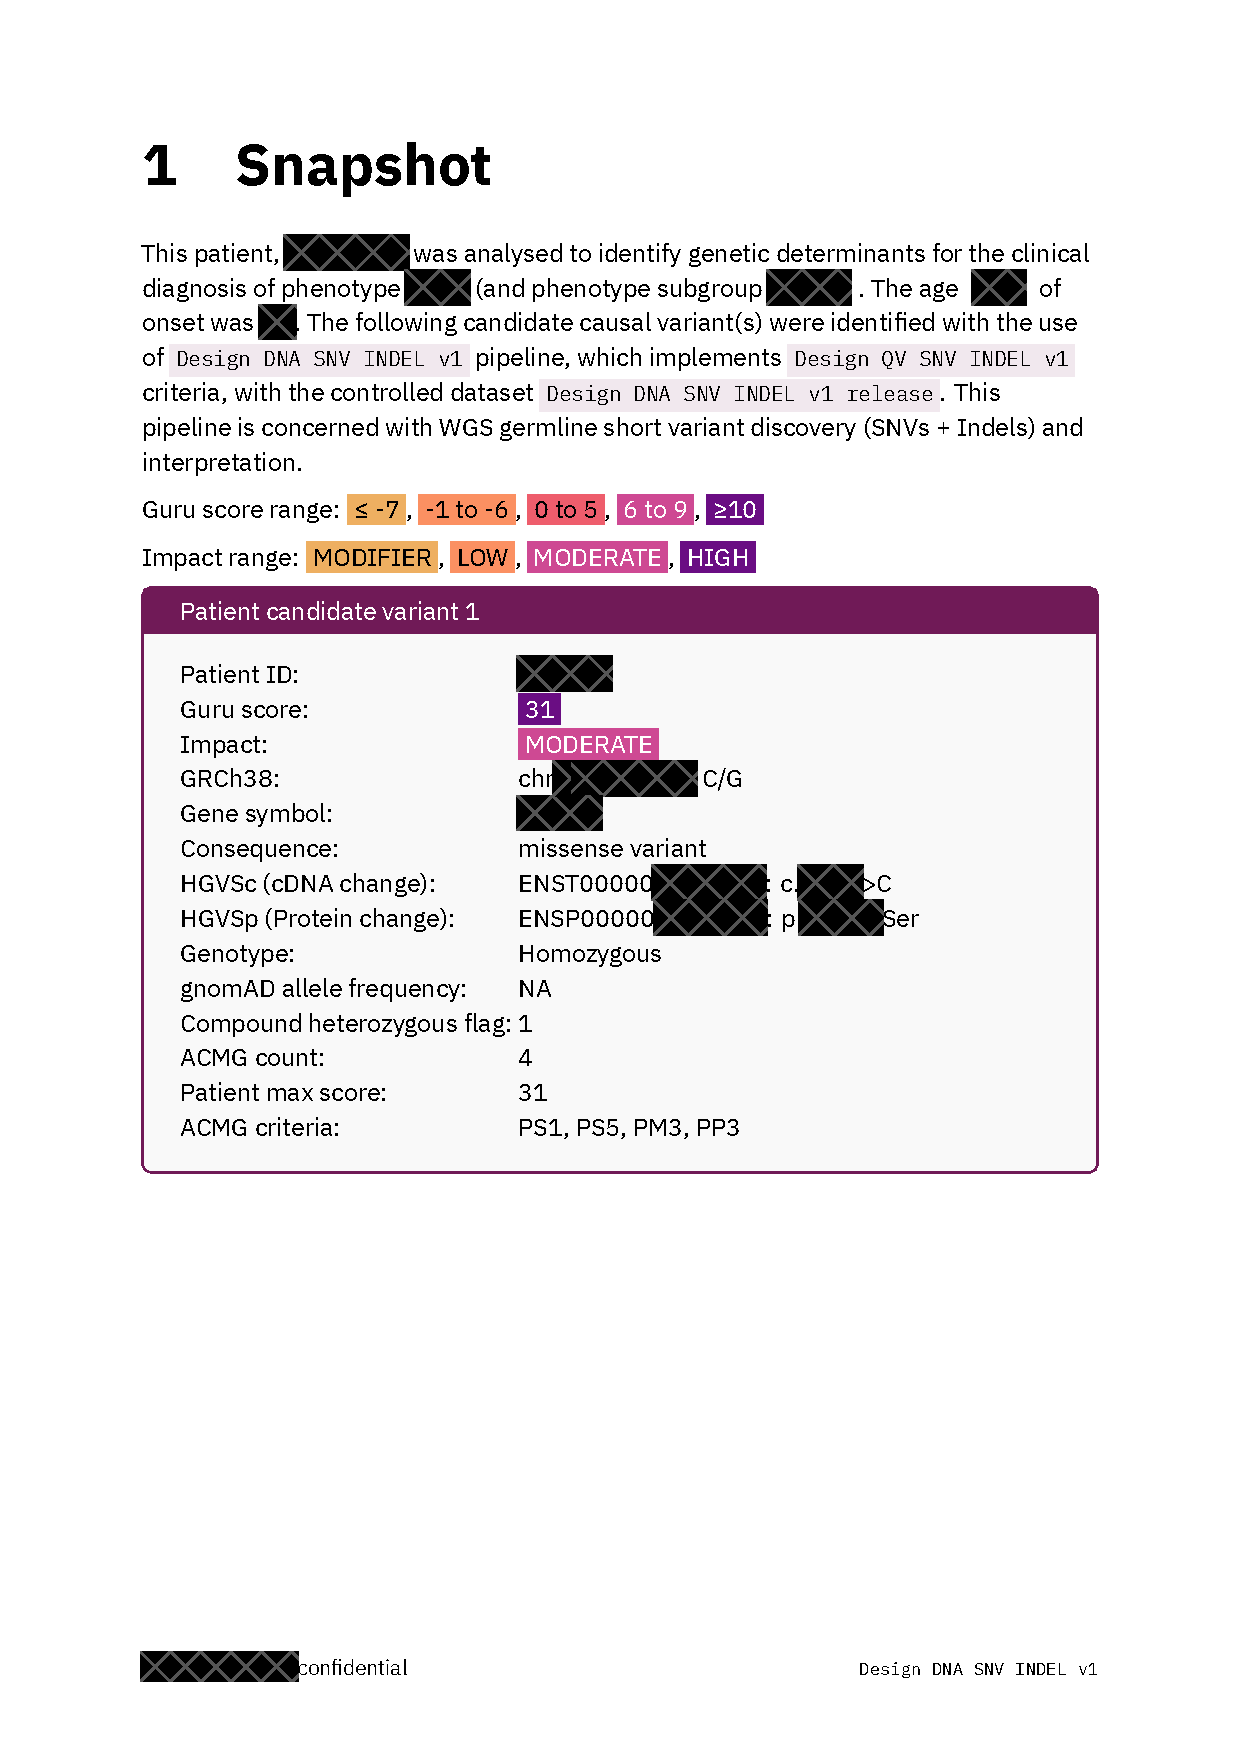
\includegraphics[width=0.32\textwidth]{sample_000_report_priority_0_1.pdf}
   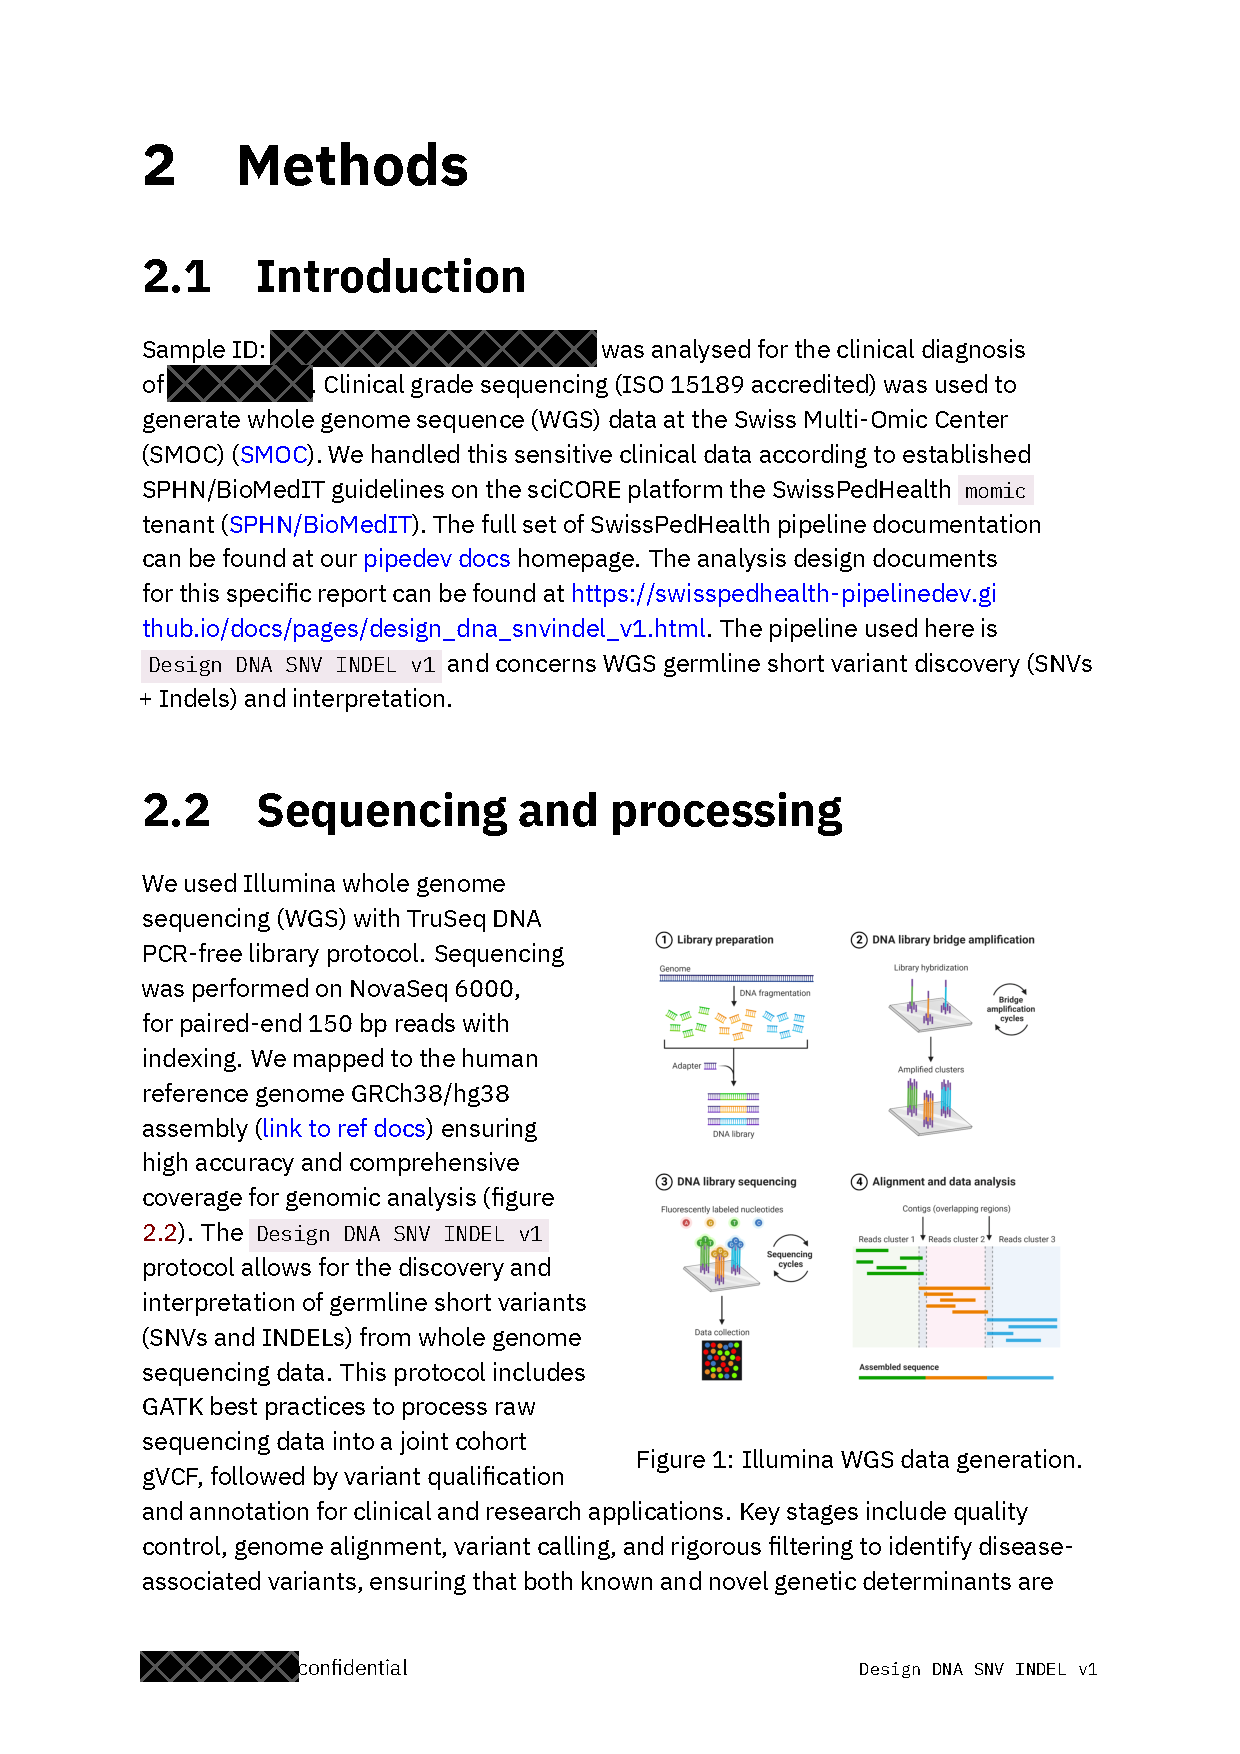
\includegraphics[width=0.32\textwidth]{sample_000_report_priority_0_2.pdf}
  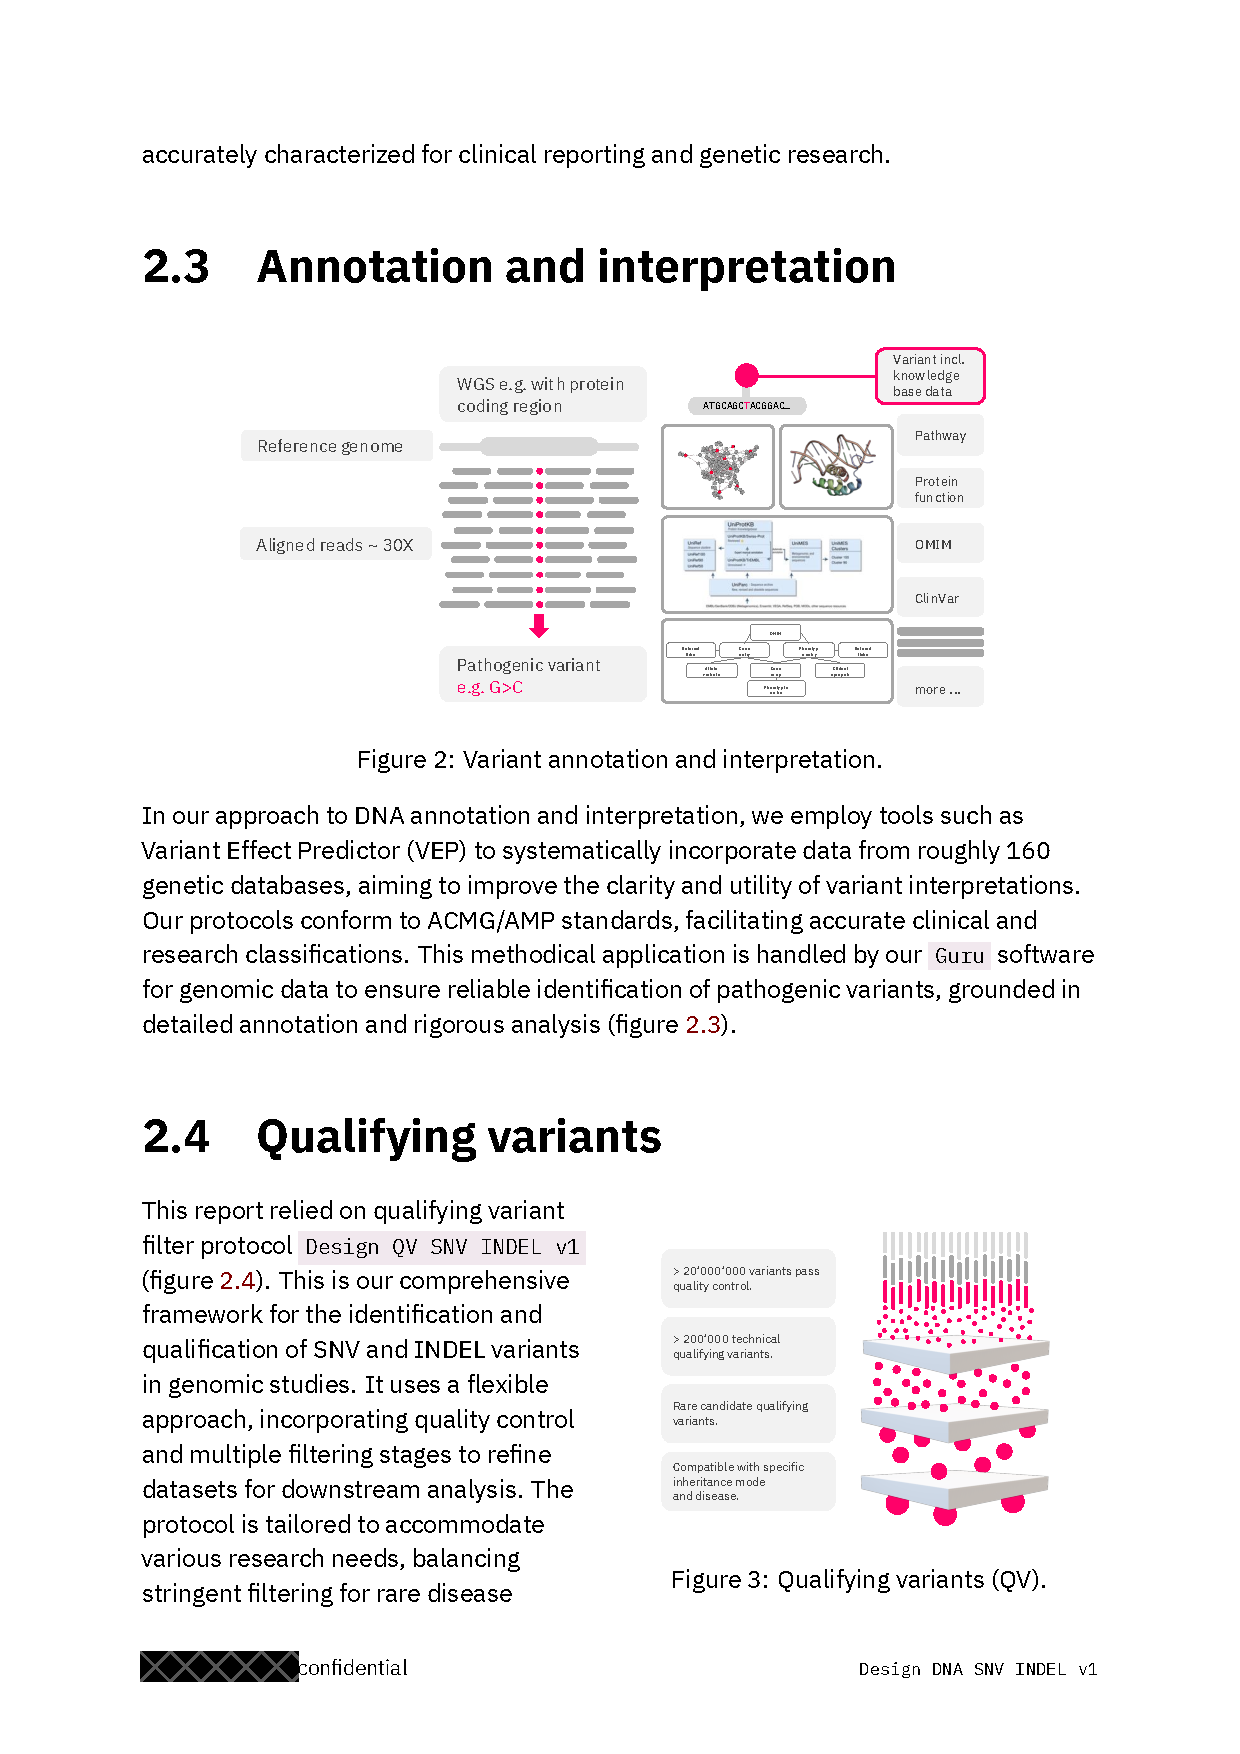
\includegraphics[width=0.32\textwidth]{sample_000_report_priority_0_3.pdf}
    \caption{Model and visual outputs generated by Dante, demonstrating efficient integration of variant annotation, ACMG scoring, other metrics.}
    \label{fig:performance}
\end{figure}


%\subsection{Integration of RAG-based Natural Language Interpretation}
%\noindent
%A novel component of our pipeline is the integration of DeepSeek-R1, accessed via the \texttt{ollamar} R package, to harness retrieval-augmented generation (RAG) for natural language interpretation of quantitative variant evidence. This process leverages detailed numerical and categorical data—such as ACMG scores, allele frequencies, and gene-specific annotations—to automatically generate an accessible narrative summary of the variant's biological and clinical significance.
%
%\noindent
%The procedure begins by aggregating quantitative evidence from multiple sources. For instance, data tables are constructed from pipeline outputs and discussion files. The R code reads variant-level metrics from a comma-separated file and discussion annotations from a tab-separated file. Selected columns, including \texttt{sample.id}, \texttt{ACMG\_total\_score}, \texttt{SYMBOL}, \texttt{HGVSc}, \texttt{HGVSp}, \texttt{Consequence}, \texttt{IMPACT}, \texttt{gnomAD\_AF} and descriptive clinical notes, are concatenated to form a comprehensive prompt.
%
%\noindent
%This prompt is augmented with predefined textual instructions that detail the structure and content required for the \emph{Evidence Interpretation Summary}. The instructions ensure that the generated text succinctly covers the biological function of the gene, its role in the disease context, and the rationale behind the pathogenic classification. By merging the quantitative evidence with these guidelines, the prompt serves as the input for the DeepSeek-R1 model.
%
%\noindent
%Using the \texttt{ollamar} package, we establish a connection with the local deployment of DeepSeek-R1. The model is queried through the \texttt{generate()} function, which streams a response containing a natural language narrative. The response is post-processed to extract the interpretable text, which is then incorporated into the final clinical report. This automated generation of narrative interpretation not only standardises the presentation of complex genomic data but also enhances its accessibility for clinical decision-making.
%
%\noindent
%In summary, the integration of DeepSeek-R1 with Ollama enables a seamless, reproducible translation of quantitative variant evidence into a coherent and concise narrative, representing a significant advancement in clinical genomics reporting.

\subsection{Integration of RAG-based Natural Language Interpretation}
\noindent
In Dante, candidate genetic variants—prioritised by tools such as GuRu based on diverse evidence sources—are filtered to fewer than ten top candidates. Given the complexity and variability of the supporting data, a retrieval-augmented generation (RAG) step is used to generate a concise, user-friendly interpretation summary. This summary, generated via the DeepSeek-R1 model through the \texttt{ollamar} R interface, translates quantitative evidence (e.g. ACMG scores, allele frequencies, gene annotations) into plain language. The process ensures that the narrative is directly supported by raw evidence, reducing the likelihood of hallucination and allowing users to rely on a quantifiable accuracy of the interpretation.


\subsection{Benchmarking and Validation}
\noindent
Benchmarking was performed using  clinical datasets of both known diagnosis and new unknown rare disease cases. Validation metrics focused on the reproducibility of ACMG-based classifications and the accuracy of candiadate variant prioritisation. Statistical measures confirmed that Dante delivers consistent performance across varying data sizes. The automated approach also minimised manual errors, thereby enhancing the overall reliability of the generated reports.

\section{Summary}
\noindent
Dante represents a significant advancement in the field of clinical genetic report generation. By automating the transformation of raw WGS data into structured, standards-compliant reports, it streamlines the workflow for clinical laboratories and genomic research facilities. The integration of detailed variant annotation, ACMG guideline adherence, and comprehensive visualisation techniques ensures that reports are both technically robust and clinically informative. Future developments will focus on integrating additional external databases and expanding the tool’s capabilities to support a broader range of genomic analyses.

\section*{Acknowledgements}
\noindent
The development of Dante was supported by colleagues at the University Children's Hospital Zürich and the University of Zürich. We thank the Swiss Multi-Omic Center for providing access to critical test datasets.

\section*{Author Contributions}
\noindent
Dylan Lawless conceived and developed the Dante pipeline, designed the study, and drafted the manuscript.

\section*{Funding}
\noindent
This work was funded by internal research grants at the University Children's Hospital Zürich and the University of Zürich.

\section*{Data Availability}
\noindent
The Dante source code, user documentation, and sample datasets are available at \url{https://github.com/DylanLawless/Dante}. Supplementary materials and further documentation can be accessed through the project repository.

\section*{Competing interest}
\noindent
We declare no competing interest. 

\clearpage
\bibliographystyle{unsrtnat}
\bibliography{references.bib}
\end{document}
